% Options for packages loaded elsewhere
\PassOptionsToPackage{unicode}{hyperref}
\PassOptionsToPackage{hyphens}{url}
%
\documentclass[
]{article}
\usepackage{lmodern}
\usepackage{amssymb,amsmath}
\usepackage{ifxetex,ifluatex}
\ifnum 0\ifxetex 1\fi\ifluatex 1\fi=0 % if pdftex
  \usepackage[T1]{fontenc}
  \usepackage[utf8]{inputenc}
  \usepackage{textcomp} % provide euro and other symbols
\else % if luatex or xetex
  \usepackage{unicode-math}
  \defaultfontfeatures{Scale=MatchLowercase}
  \defaultfontfeatures[\rmfamily]{Ligatures=TeX,Scale=1}
\fi
% Use upquote if available, for straight quotes in verbatim environments
\IfFileExists{upquote.sty}{\usepackage{upquote}}{}
\IfFileExists{microtype.sty}{% use microtype if available
  \usepackage[]{microtype}
  \UseMicrotypeSet[protrusion]{basicmath} % disable protrusion for tt fonts
}{}
\makeatletter
\@ifundefined{KOMAClassName}{% if non-KOMA class
  \IfFileExists{parskip.sty}{%
    \usepackage{parskip}
  }{% else
    \setlength{\parindent}{0pt}
    \setlength{\parskip}{6pt plus 2pt minus 1pt}}
}{% if KOMA class
  \KOMAoptions{parskip=half}}
\makeatother
\usepackage{xcolor}
\IfFileExists{xurl.sty}{\usepackage{xurl}}{} % add URL line breaks if available
\IfFileExists{bookmark.sty}{\usepackage{bookmark}}{\usepackage{hyperref}}
\hypersetup{
  pdftitle={Dataset: TED TALKS},
  pdfauthor={Blanch Torras, Rem},
  hidelinks,
  pdfcreator={LaTeX via pandoc}}
\urlstyle{same} % disable monospaced font for URLs
\usepackage[margin=1in]{geometry}
\usepackage{graphicx,grffile}
\makeatletter
\def\maxwidth{\ifdim\Gin@nat@width>\linewidth\linewidth\else\Gin@nat@width\fi}
\def\maxheight{\ifdim\Gin@nat@height>\textheight\textheight\else\Gin@nat@height\fi}
\makeatother
% Scale images if necessary, so that they will not overflow the page
% margins by default, and it is still possible to overwrite the defaults
% using explicit options in \includegraphics[width, height, ...]{}
\setkeys{Gin}{width=\maxwidth,height=\maxheight,keepaspectratio}
% Set default figure placement to htbp
\makeatletter
\def\fps@figure{htbp}
\makeatother
\setlength{\emergencystretch}{3em} % prevent overfull lines
\providecommand{\tightlist}{%
  \setlength{\itemsep}{0pt}\setlength{\parskip}{0pt}}
\setcounter{secnumdepth}{-\maxdimen} % remove section numbering

\title{Dataset: TED TALKS}
\author{Blanch Torras, Rem}
\date{13 de Abril de 2020}

\begin{document}
\maketitle

\hypertarget{descripciuxf3n}{%
\subsection{Descripción}\label{descripciuxf3n}}

El conjunto de datos generado como parte de esta actividad práctica
reúne diferentes características de las charlas realizadas en los
eventos de TED.

TED es una organización sin fines de lucro dedicada al concepto ``Ideas
que vale la pena difundir''.

En una conferencia TED, se les pide a los principales pensadores y
hacedores del mundo que den su discurso en 18 minutos o menos. Los
oradores de TED han incluido a Roger Ebert, Sheryl Sandberg, Bill Gates,
Elizabeth Gilbert, Benoit Mandelbrot, Philippe Starck, Ngozi
Okonjo-Iweala, Brian Greene, Isabel Allende y el ex primer ministro
británico Gordon Brown.

En TED.com, las charlas de las conferencias de TED se comparten con el
mundo de forma gratuita como videos de TED Talks. A través del Proyecto
de traducción abierta, las charlas TED son subtituladas por voluntarios
de todo el mundo en más de 90 idiomas.

Algunas de las variables que se recogen en el conjunto de datos son la
fecha, el tema, los ponentes, el número de visitas o o los idiomas
disponibles.

\hypertarget{imagen-identificativa}{%
\subsection{Imagen identificativa}\label{imagen-identificativa}}

\begin{figure}
\centering
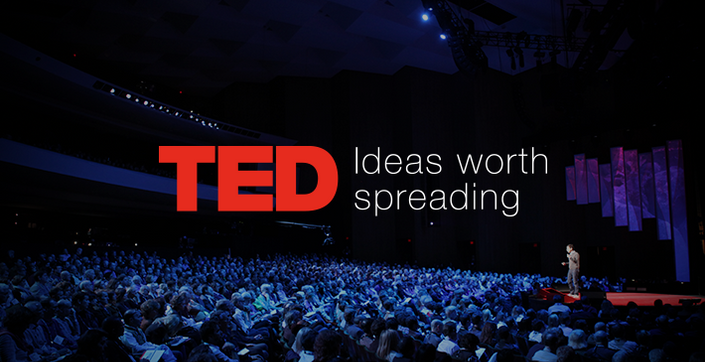
\includegraphics{./TED_banner.png}
\caption{TED TALKS}
\end{figure}

\hypertarget{contexto}{%
\subsection{Contexto}\label{contexto}}

Como se ha comentado, la materia del conjunto de datos se corresponde
con las charlas realizadas en las conferencias TED y subidas a la página
web de dicha organización.

\hypertarget{contenido}{%
\subsection{Contenido}\label{contenido}}

Para cada accidente, el cual se corresponde con un registro en el
conjunto de datos, se recogen las siguientes características:

\begin{itemize}
\tightlist
\item
  \textbf{posted\_date}: Fecha de publicación en el formato
  dd-mm-aaaa.\\
\item
  \textbf{update\_date}: Fecha de realización del proceso de web
  scraping.\\
\item
  \textbf{talk\_title}: Título de la presentación.\\
\item
  \textbf{talk\_description}: Descripción del tema de la presentación.\\
\item
  \textbf{talk\_main\_speaker}: Principal ponente de la presentación.\\
\item
  \textbf{talk\_speakers\_info}: Nombre y enlace a los perfiles de los
  ponentes..\\
\item
  \textbf{talk\_link\#}: Enlace al vídeo de la presentación.\\
\item
  \textbf{talk\_lang}: Idioma de la presentación.\\
\item
  \textbf{available\_languages}: Idiomas disponibles en las
  transcripciones de la presentación.\\
\item
  \textbf{talk\_topics}: Principales temas de la presentación.\\
\item
  \textbf{talk\_duration}: Duración total de la presentación.\\
\item
  \textbf{talk\_trancript}: Transcripción de la presentació.
\item
  \textbf{talk\_upload\_video\_date}: Fecha de subida del vídeo de la
  presentación.\\
\item
  \textbf{talk\_views}: Total de visitas de la ponencia.
\end{itemize}

\hypertarget{agradecimientos}{%
\subsection{Agradecimientos}\label{agradecimientos}}

Los datos han sido recolectados desde la página principal de
\href{https://www.ted.com/talks}{TED}. Para ello, se ha hecho uso del
lenguaje de programación Python y de técnicas de \emph{Web Scraping}
para extraer la información alojada en las páginas HTML.

\hypertarget{inspiraciuxf3n}{%
\subsection{Inspiración}\label{inspiraciuxf3n}}

El presente conjunto de datos podría utilizarse en ámbitos muy diversos.

Debido a la popularidad de las charlas educativas, podria utilizares
para generar un repositorio de conferencias junto a otros eventos como
pueden ser los de \href{https://99u.adobe.com/}{\emph{99U}},
\href{https://creativemornings.com/}{\emph{Creative Mornings}} o las
\href{https://talksat.withgoogle.com/}{\emph{Google Talk}}.

También podria ser interesante expandir dicho proyecto orientandolo a la
\emph{mineria de datos}. Realizando un análisis en mayor profundidad
extrayendo, por ejemplo, los comentarios y las valoraciones de los
usuarios, se podria valorar cuales son los temas de mayor relevancia
según franja de edad, género y campo de estudio así como qué tipo de
presentación recibe mejor aceptación y en qué momento se genera un
ambiente de discordia.

\hypertarget{licencia}{%
\subsection{Licencia}\label{licencia}}

La licencia elegida para la publicación de este conjunto de datos ha
sido \textbf{CC BY-SA 4.0 License}. Los motivos que han llevado a la
elección de esta licencia tienen que ver con la idoneidad de las
cláusulas que esta presenta en relación con el trabajo realizado:

\begin{itemize}
\item
  \emph{Reconocimiento} --- Se debe reconocer adecuadamente al autor,
  proporcionado un enlace a la licencia e indicar si se han realizado
  cambios.
\item
  \emph{CompartirIgual} --- Si se realiza cualquier tipo de trabajo
  sobre este proyecto, es necesarop difundir dichas contribuciones bajo
  la misma licencia que el original.
\end{itemize}

\hypertarget{cuxf3digo-fuente-y-dataset}{%
\subsection{Código fuente y dataset}\label{cuxf3digo-fuente-y-dataset}}

Tanto el código fuente escrito para la extracción de datos como el
dataset generado pueden ser accedidos a través de
\href{https://github.com/Rem-Blanch/Web-scraping-TED}{este enlace}.

\hypertarget{recursos}{%
\subsection{Recursos}\label{recursos}}

\begin{enumerate}
\def\labelenumi{\arabic{enumi}.}
\tightlist
\item
  Lawson, R. (2015). Web Scraping with Python. (2nd ed.). : Packt
  Publishing Ltd.
\item
  Mitchell, R. (2015). Web Scraping with Python: Collecting Data from
  the Modern Web. (2nd ed.). : O'Reilly Media, Inc.
\item
  Tagliaferri, L. (2019). Digital Ocean. Retrieved 07 April, 2020, from
  \url{https://www.digitalocean.com/community/tutorials/how-to-scrape-web-pages-with-beautiful-soup-and-python-3}
\item
  Richardson, L. (2004). Beautiful Soup documentation. Retrieved 07
  April, 2020, from
  \url{https://www.crummy.com/software/BeautifulSoup/bs4/doc/}
\item
  Miller, W. (2018). William Miller's Projects. Retrieved 12 April,
  2020, from \url{https://wamiller0783.github.io/TED-scraping-post.html}
\end{enumerate}

\end{document}
